\documentclass[11pt]{scrartcl}
\usepackage[utf8]{inputenc} % Kodierung der Textdatei mit Sonderzeichen
\usepackage[ngerman]{babel} % Sprache fuer Inhaltsverzeichnis etc.
\usepackage{amssymb} % Mathematische Symbole
\usepackage{amsmath} % Mehr mathematische Konstrukte
\usepackage{graphicx} % Um Bilder einbinden zu koennen
\usepackage{float} % fuer \begin{figure}[H]
\usepackage{icomma} % laesst das Komma als Dezimaltrennzeichen interpretieren
\usepackage{fix-cm} % für die große Titelschrift
\usepackage{placeins} % laesst Bilder nicht über eine \FloatBarrier hinausrutschen
\usepackage[pdftex]{hyperref} % Hyperlinks im Dokument
\hypersetup{colorlinks=true, linkcolor=black, citecolor=black, filecolor=black, urlcolor=black, pdftitle={Erdrotationsmessung - Projektpraktikum 09/10 Gruppe 5}}


\newcommand{\unit}[1]{\ensuremath{\,\mathrm{#1}}} % Einheiten schreiben sich immer aufrecht!
\newcommand{\degr}{\ensuremath{^\circ}}
\newcommand{\cel}{\ensuremath{\degr\mathrm{C}}}
\newcommand{\dif}{\ensuremath{\mathrm{d}}}
\newcommand{\pdif}[2]{\ensuremath{\frac{\partial#1}{\partial#2}}}
\newcommand{\ee}[1]{\ensuremath{\cdot 10^{#1}}}
\newcommand{\ltext}[1]{\ensuremath{_{\textnormal{#1}}}}
\newcommand{\hypref}[2]{\hyperref[#2]{{#1}~\ref{#2}}}

\setlength{\parindent}{1em}
\setlength{\parskip}{0.5\baselineskip}

\graphicspath{{images/}}


\title{Direkte Messung der Erdrotation - Gruppe 5 WS 09/10, Projektpraktikum der Uni Erlangen}
\date{07.12.2009 -- 15.01.2010}
\author{Michele Collodo, Andreas Glossner, Karl-Christoph G\"odel, Bastian Hacker, Maria Obst, Alexander Wagner, David Winnekens}



\begin{document}
\sloppy % laesst Latex nicht ueber den Rand rausschreiben
\thispagestyle{empty}
\large{Projektpraktikum WS 09/10}
\hfill
\raisebox{-1.4cm}{
\includegraphics[width=5cm]{fau.pdf}}
\\[8\baselineskip]
\begin{center}
{\fontsize{36}{54}\textbf{Direkte Messung der Erdrotation}}
\\[2\baselineskip]
{\Large 07.12.2009 -- 15.01.2010}
\\[7\baselineskip]
{\huge\textbf{PPG 5}}
\\[0.5\baselineskip]
{\large\textbf{
Michele Collodo,
Andreas Glossner,\\
Karl-Christoph G\"odel,
Bastian Hacker,\\
Maria Obst,
Alexander Wagner,
David Winnekens}\\
Tutor: Xiaoyue Jin}
\vfill



\small{\url{http://pp.physik.uni-erlangen.de/groups/ws0910/ppg5/ppg5\_start.html}}
\end{center}
\newpage



\tableofcontents
\vfill



\begin{abstract}
In diesem Projekt wurde versucht, die Drehgeschwindigkeit der Erde im Labor zu messen.
Hierzu wurde eine massive, drehbar gelagerte Stange verwendet, die ihr Trägheitsmoment um die vertikale Achse durch Einklappen um den Faktor 3600 ändern kann und damit die vorhandene Drehbewegung verstärkt und messbar macht.
Im Gegensatz zum Foucaultschen Pendel ist hiermit eine instantane Messung möglich.
Allerdings hatten wir mit starken Schwingungs- und Reibungseffekten zu kämpfen, so dass unsere Werte am Ende immer noch um eine Größenordnung daneben lagen.
\end{abstract}
\newpage

\section{Einleitung} %Michele
Die Länge eines Tages, also die Zeit, die die Erde benötigt, um sich um die eigene Rotationsachse zu drehen, ist die älteste zeitliche Maßeinheit, von welcher ausgehend unser modernes Zeitsystem abgeleitet wurde. Auch wenn heute die Sekunde nicht mehr über die Erddrehung definiert ist, so ist die präzise Kenntnis der Rotationsdauer der Erde in vielen Bereichen, allen voran der Astronomie, von großer Bedeutung. Bezogen auf den kosmischen Hintergrund beträgt diese 86\,164.1 Sekunden (mittlerer siderischer Tag).

Die wohl älteste Methode zur Bestimmung dieser Rotationsgeschwindigkeit ist die Beobachtung des Sonnenstandes.
Bei dieser Messung muss aber zwingend berücksichtigt werden, dass sich die Erde nicht nur um sich selbst, sondern auch um die Sonne dreht, eine Erdumdrehung also geringfügig länger dauert, als die Zeitspanne zwischen zwei Kulminationen der Sonne. Umgehen kann man diesen Effekt, wenn man direkt einen Fixstern beobachet, heutzutage werden hierfür extragalaktische Radioquellen herangezogen. Eine ebenfalls gebräuchliche Vorgehensweise ist die Positionsbestimmung geeigneter Satelliten.

Eine weitere Möglichkeit der Messung der Winkelgeschwindigkeit der Erde kann über die rotationsbedingten Scheinkräfte, also der Zentrifugal- und der Corioliskraft, erfolgen. Besonders anschaulich ist hierbei das Foucaultsches Pendel, möglich ist aber auch die Messung des Gewichtsunterschiedes eines Körpers an verschiedenen Breitengraden der Erde, der es unter Berücksichtigung der lokalen Fallbeschleunigungen erlaubt, auf die Zentrifuaglkraft zu schließen. 

Wir haben uns, besonders wegen der Durchführbarkeit in einem kleinen und abgedunkelten Labor, für eine unkonventionelle Messmethode entschieden. Hierzu machen wir uns den Drehimpulserhalt sowie die Variation des Tr\"agheitsmoments unserer Messvorrichtung zunutze.

\section{Grundprinzip - Tr\"agheitsmoment}\label{sec:grundprinzip}
\begin{figure}[th]
\begin{center}
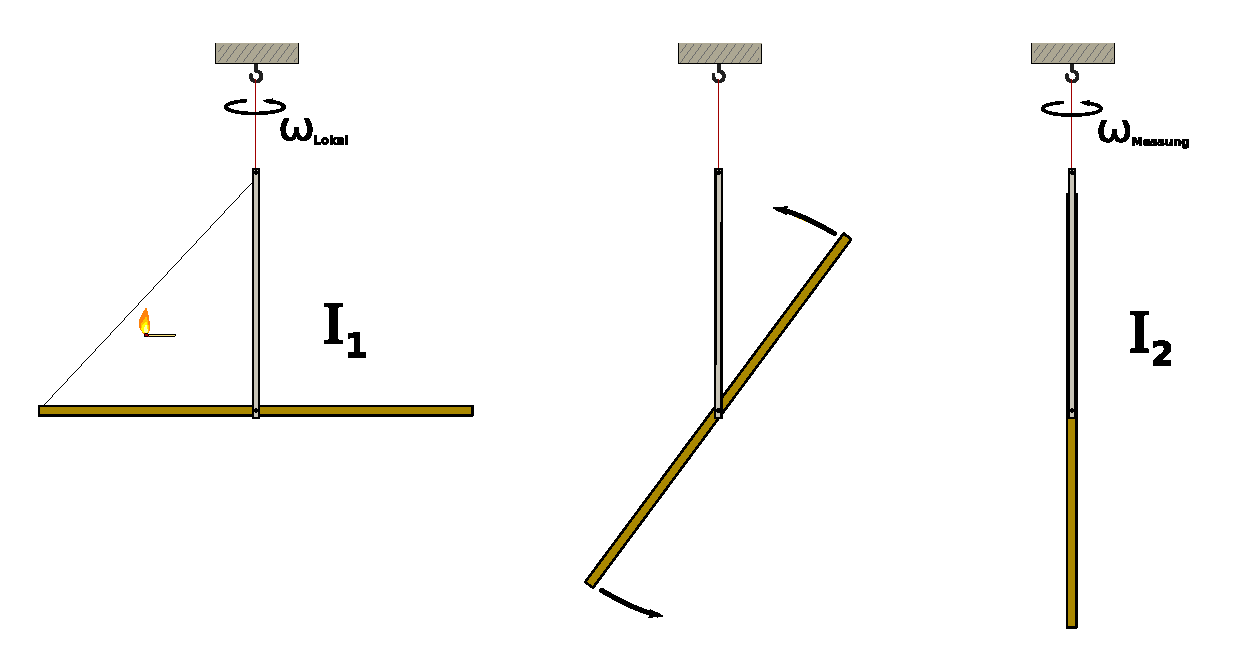
\includegraphics[width=0.8\textwidth]{prinzip.pdf}
\end{center}
\vspace{-1.5\baselineskip}
\caption{Schema des Bewegungsablaufs}
\label{prinzip}
\end{figure}
Unter Ausnutzung der Drehimpulserhaltung wurde mit dem in den \hypref{Abbildungen}{prinzip} und\hypref{}{Welt} skizzierten Aufbau versucht die Erdrotationsdauer zu bestimmen. Ein drehbar gelagerter, massiver Messingstab wurde dabei frei an einem Faden im Labor aufgeh\"angt. Der aufgeklappte Stab dreht sich nach einer gewissen Zeit (einigen Stunden) mit der Erde mit, da dann Torsionseffekte durch den Faden, etc. keine Rolle mehr spielen. L\"asst man den Stab in seine Ausgangslage zur\"uckklappen, so muss der Drehimpuls erhalten bleiben. Misst man nun die Rotationsdauer des Systems, kann man daraus die Erdrotationsdauer ermitteln:
Befindet man sich an einem Ort mit Breitengrad $\alpha$, so gilt aufgrund der Drehimpulserhaltung (hierbei bezeichnet $I\ltext{parallel}$ das Tr\"agheitsmoment des Systems im hochgeklappten Zustand und $I\ltext{senkrecht}$ das Tr\"agheitsmoment im ausgelenkten Zustand):
\begin{eqnarray}
L_1 &=& L_2 \\
\omega\ltext{Erde}\cos\alpha \cdot I\ltext{senkrecht} &=&
\omega\ltext{dreh} \cdot I\ltext{parallel} \\
&=& (\omega\ltext{mess} + \omega\ltext{Erde}\cos\alpha) \cdot I\ltext{parallel}
\end{eqnarray}
Damit ergibt sich schließlich die Erdrotationsdauer:
\begin{equation}
\label{eq:grund}
\boxed{
\omega\ltext{Erde} =
\frac{1}{\cos\alpha}\ 
\frac{\omega\ltext{mess}}{I\ltext{senkrecht} / I\ltext{parallel} - 1}
}
\end{equation}

\begin{figure}[ht]
\begin{center}
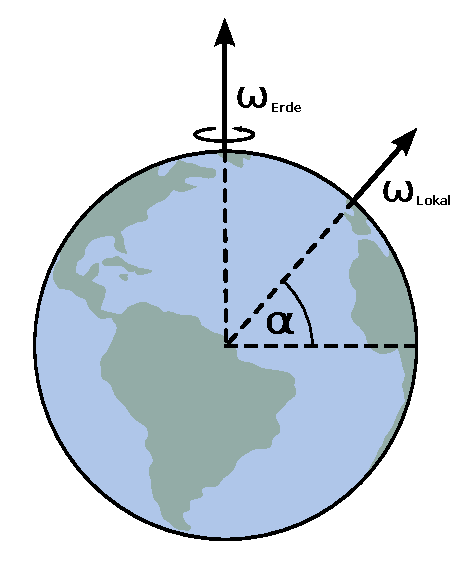
\includegraphics[width=0.3\textwidth]{welt.pdf}
\end{center}
\vspace{-1.5\baselineskip}
\caption{Position auf der Erde}
\label{Welt}
\end{figure}

%\FloatBarrier
\section{Bau des Drehstabs} %Maria (solltest du nicht zu allem was wissen, sag bescheid)

%%% Ich hab jetzt mal alles reingeschrieben was ich wusste. Mit den subsections bin ich nicht ganz klar gekommen in der Form, drum habe ich die weggelassen, aber ich denke es ist trotzdem alles drin was rein sollte. Wo Fragezeichen stehen war ich mir nicht sicher bzw. wusste keine konkreten Werte. Bei weiteren Beschwerden bitte bei mir meckern :)

Der im Experiment verwendete Drehstab wurde in mehreren Schritten weiter verbessert. Das Ger\"ust jeder der Versionen war die Gabel, in der die drehbar gelagerte Stange aufgeh\"angt wurde. Zwei d\"unnwandige Aluminiumzylinder der L\"ange 91,8 \unit{cm} mit einem Durchmesser von $1\unit{cm}$ und einer Wandstärke von $1,2\unit{mm}$ sowie einer Masse von jeweils $66,5\pm 0,14\unit{g}$ dienten als Stabilisator für den drehbaren Stab. Die beiden Gabelstangen wurden von zwei Achsen parallel gehalten: Die Untere diente gleichzeitig als Drehachse f\"ur den Drehstab, an der Oberen wurde die Anordnung an einer Halterung an der Decke des Raumes aufgeh\"angt. Hierf\"ur wurde Nylonfaden der St\"arke $0,7\unit{mm}$
% ist 4mm nicht etwas dick für den Faden ??? - Ja; Habe mal 0,7mm daraus gemacht, das erscheint mir realistischer, oder?!
 verwendet, um einerseits eine m\"oglichst d\"unne unverdrillte Aufh\"angung zu gew\"ahrleisten, welche die Rotation nicht beeinflusst und andererseits das Gewicht des Drehstabes zuverl\"assig zu halten. Zudem waren an der oberen Achse d\"unne Balsaholzstreifen angebracht, die bei der Drehung des Stabes durch die Lichtschranken liefen. Ein Anglerwirbel zwischen Nylonfaden und Stab erwieß sich als nicht sinnvoll, da er aufgrund der Reibung durch das große Gewicht des Stabes nicht drehte sondern blockierte.

In der Gabel wurde zun\"achst ein Drehstab aus massivem Stahl aufgeh\"angt. Dieser hatte eine L\"ange von 1,70 \unit{m}, einen Radius von $6,0\pm 0,05\unit{mm}$ sowie ein Gewicht von $1,5\pm 0,3\unit{kg}$. Die waagrechte Rotationsachse des Stabes lag dabei nicht in dessen Schwerpunkt. Mithilfe von N\"ahgarn wurde das schwerere Ende des Stabes hochgebunden und dieser somit in eine waagerechte Position gebracht. So wurde sicher gestellt, dass er sich nach Durchbrennen des Fadens senkrecht ausrichtet.

Um zu verhindern, dass der Stab \"uber die Senkrechte hinausschwingt, wurde eine Bremse aus Styropor am oberen Ende der Gabel angebracht. F\"ur ein sicheres Einrasten in die Senkrechte sorgte ein in die Bremse eingeschobener Magnet der Masse $24,0 \pm 0,3\unit{g}$. Um den Stab gen\"ugend zu beschleunigen, sodass er schnell und fest einrastet, wurde ein Federmechanismus aus Draht und Gummi an der Drehachse angebracht. %(siehe \hyperref[zugmechanismus]{Abb.~\ref{zugmechanismus}}) 
%\begin{figure}[ht]
%\begin{center}
%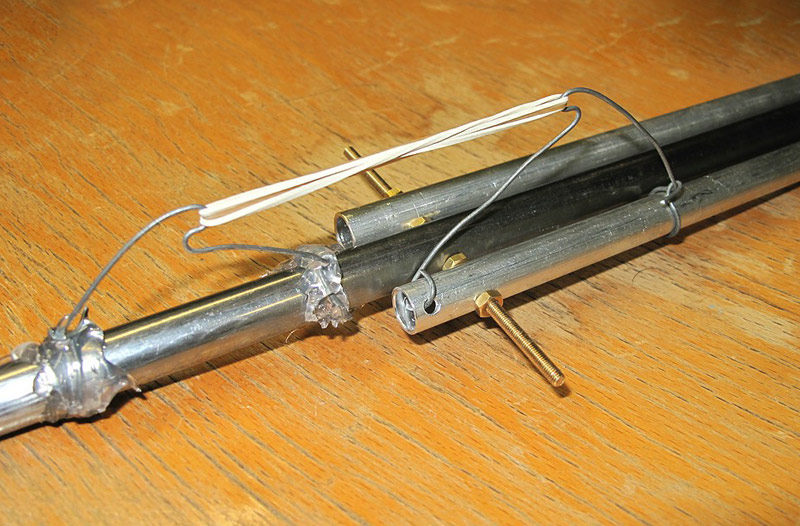
\includegraphics[width=0.8\textwidth]{zugmechanismus.jpg}
%\end{center}
%\vspace{-1.5\baselineskip}
%\caption{Gummizug zum Einklappen des Stabes}
%\label{zugmechanismus}
%\end{figure}
%
%%%%%%%%%% Bild notwendigtig? - Axi ; denke nicht - David

Nach den ersten Versuchen mit diesem Aufbau zeigte sich, dass beim Hochklappen des Stabes der Nylonfaden der Aufh\"angung stark zu schwingen begann. Um den Einfluss dieser Schwingung auf die zu messende Rotation m\"oglichst gering zu halten und um zu vermeiden, dass die Balsaholzst\"abe nicht mehr durch die Lichtschranken laufen, wurde der Nylonfaden sp\"ater durch ein Plexiglasr\"ohrchen gef\"uhrt, welches am Gerüst der Lichtschranken befestigt war. Jedoch war auch dieser Aufbau fehleranf\"allig, da die Reibung zwischen Faden und Rohr die Rotation beeintr\"achtigte.

Nach einigen fehlgeschlagenen Versuchen stellten wir fest, dass der eingebaute Halterungsmagnet, sowie die leicht magnetisierte Eisenstange selbst als Kompass im Erdmagnetfeld fungierten und somit die empfindliche Messung erheblich störten.
Einerseits konnte damit der Faden auch nach längerer Wartezeit keine drehmomentfreie Lage einnehmen, andererseits störte das magnetische Drehmoment den Stab während der Messung.
Um s\"amtliche Einfl\"usse von Magnetfeldern auszuschalten, wurde nicht nur der ferromagnetische Eisenstab durch einen ansonsten baugleichen Messingstab der Masse 1,5\unit{kg} ersetzt, sondern auch der Magnet in der Bremse gegen einen Klettverschluss ausgetauscht, dessen Gegenst\"uck am oberen Drehstabende befestigt wurde. Zuletzt wurden noch die zwei Balsaholzst\"abchen, die die Lichtschranke ausl\"osen sollten, mit einen Kranz aus 36 St\"abchen im Abstand von jeweils 10$^{\circ}$ ausgewechselt, um mehr Messpunkte zu erhalten.

%\subsection{Material}
%Magnetismus, Verwindung usw.
%\subsection{Aufh\"angung}
%Stabilisierung der Drehbewegung
%\subsection{Klappmechanismus}
%Zugmechanismus, Einrasten

\begin{figure}[ht]
\begin{center}
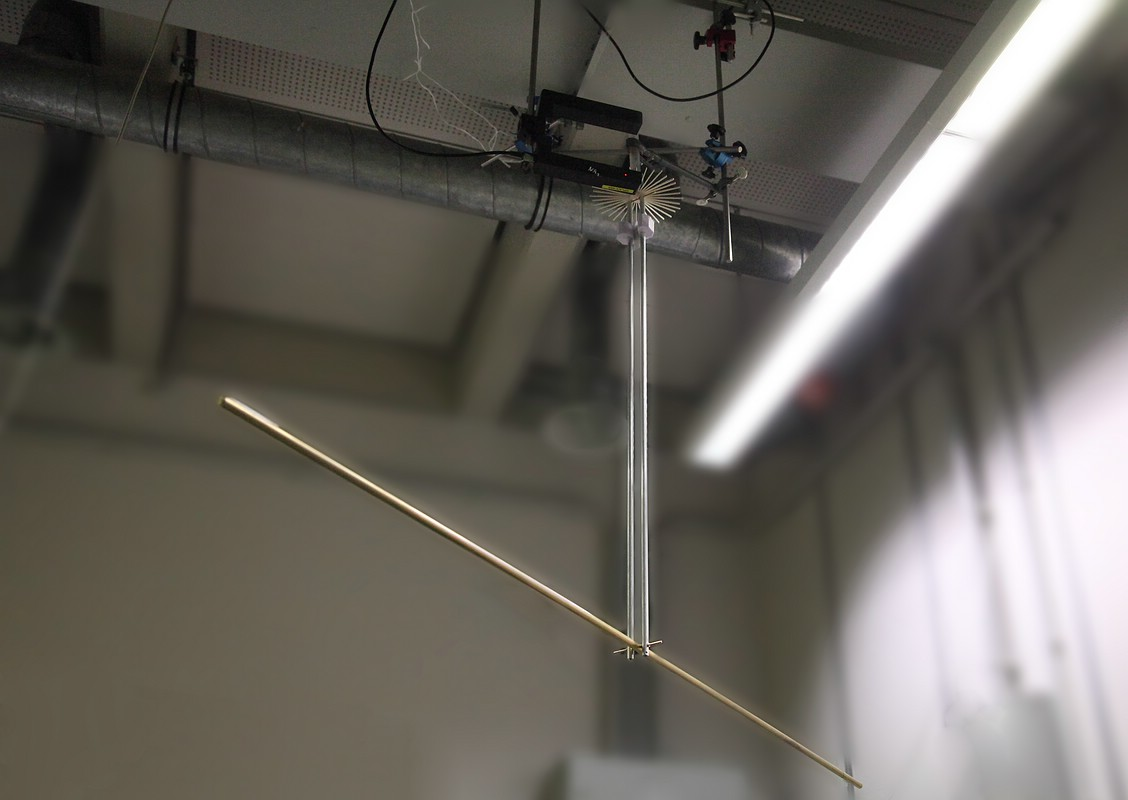
\includegraphics[width=0.8\textwidth]{stab-fertig.jpg}
\end{center}
\vspace{-1.5\baselineskip}
\caption{Der ausgelenkte Stab}
\label{stab-fertig}
\end{figure}

\section{Messungen}
\subsection{Berechnungen im Voraus} %Andi

\subsubsection{Berechnung der theoretischen Rotationsdauer des zugeklappten Aufbaus}

Zun\"achst wurde die Rotationsdauer des Aufbaus nach dem Hochklappen des Messingsstabes (d.h. im "`parallelen Zustand"') rechnerisch bestimmt. 

Der erste Schritt dabei war die Berechnung der Tr\"agheitsmomente. Dazu wurden die folgenden geometrischen N\"aherungen vorgenommen:

\begin{tabular}[ht]{|l|c|}
  \hline
  Ann\"aherung in Rechnung & Objekt im Aufbau\\
  \hline\hline
	Vollzylinder & Messingstange (Mittelstange)\\
	Hohlzylinder & Aluminiumstangen (Befestigung)\\
	d\"unner, langer Stab & kleine Gewindestangen (Befestigung%; Achse und Befestigung Klettverschluss
)\\
	Quader & Magnet (1. Aufbau; sp\"ater stattdessen Klettverschluss)\\
  \hline
\end{tabular}


\noindent
Es gilt also:
\begin{equation}
I\ltext{Vollzylinder-parallel}
=\frac{1}{2} \cdot (R\ltext{Vollzylinder})^2 \cdot M\ltext{Vollzylinder}
\end{equation}
\begin{eqnarray}
I\ltext{Vollzylinder-senkrecht}
&=& \frac{1}{12} \cdot (L\ltext{Vollzylinder})^2 \cdot M\ltext{Vollzylinder}\nonumber\\
&& + (a\ltext{Vollzylinder})^2 \cdot M\ltext{Vollzylinder}
\end{eqnarray}
\begin{eqnarray}
I\ltext{Hohlzylinder}
&=&\frac{1}{2} \cdot M\ltext{Hohlzylinder} \cdot ((R\ltext{innen})^2+(R\ltext{außen})^2)\nonumber\\
&& +(a\ltext{Hohlzylinder})^2 \cdot M\ltext{Hohlzylinder}
\end{eqnarray}
\begin{equation}
I\ltext{dünner, langer Stab}
=\frac{1}{12} \cdot M\ltext{dünner, langer Stab} \cdot L^2
\end{equation}
%Fehlt: Erklärung was die "a_..." sind und deren Werte
Hierbei beschreibt $ a\ltext{Vollzylinder} = 0,8 \unit{cm} $ den Abstand des Aufh�ngepunktes des Messingstabes von seinem Schwerpunkt und $ a\ltext{Hohlzylinder} = 1,4 \unit{cm} $ die Entfernung der zwei Hohlzylinder von der Drehachse.\\
Daraus ergibt sich mit den obigen Werten bei der Messung mit Klettverschluss und Messingstab (der Klettverschluss wurde bei den Rechnungen vernachl"assigt):\\
\\
In senkrechter Position:
\begin{eqnarray}
I\ltext{Aufbau-senkrecht}=I_1
&=&
I\ltext{Vollzylinder-senkrecht}+2 \cdot I\ltext{Hohlzylinder} + 2 \cdot I\ltext{dünner, langer Stab}\nonumber\\
&=& 3,6 \ee{-1} \unit{kg} \unit{m^2}
\end{eqnarray}
In paralleler Position (nach dem Zuklappen):
\begin{eqnarray}
I\ltext{Aufbau-parallel}=I_2
&=& I\ltext{Vollzylinder-parallel}+2 \cdot I\ltext{Hohlzylinder} + 2 \cdot I\ltext{dünner, langer Stab}\nonumber\\
&=& 9,9 \ee{-5} \unit{kg} \unit{m^2}
\end{eqnarray}
Daraus ergibt sich zusammen mit \hypref{Gleichung}{eq:grund}
%\begin{equation}
%\omega\ltext{mess} = 
%\cos\alpha \cdot (I\ltext{senkrecht} / I\ltext{parallel} - 1) \cdot \omega\ltext{Erde}
%\end{equation}
%Referenz reicht - würde ich sagen ?!
die Periodendauer einer Drehung nach dem Hochklappen zu
\begin{equation}
\label{eq:tpara}
T_{parallel}=30,3 \unit{s}.
\end{equation}
Der tats"achlich gemessene Wert war jeweils betr"achtlich k"urzer - die vermuteten Gr"unde hierf"ur sind weiter unten angegeben.

\subsubsection{Berechnung der Erdrotationsdauer aus der gemessenen Rotationsdauer des zugeklappten Aufbaus}

Die eigentliche Grundidee des Versuchs war es nat\"urlich, die Erdrotationsdauer aus dem \textit{gemessenen} Wert f\"ur die Rotationsdauer des zugeklappten Aufbaus experimentell zu bestimmen. Die Rechnung und Herleitung dazu finden sich unter dem obigen \hypref{Abschnitt}{sec:grundprinzip}:

\begin{equation}
\omega\ltext{Erde} = 
\frac{1}{\cos(40,4\degr)}\ 
\frac{\omega\ltext{mess}}{(3,6\ee{-1}) / (9,9\ee{-5}) - 1}
= \frac{1}{4\,904\unit{s}} %% stimmt der Wert jetzt noch?, wie gro� ist hier omega-mess? by Axi
\end{equation}

Mit unseren vorweggenommenen Messwerten w"urde sich folglich eine Rotationsdauer von 4\,904\unit{s} ergeben -- also ein deutlich k"urzerer Wert als ein Tag!

\subsection{Cassymessungen} %Axi
\begin{figure}[ht]
\begin{center}
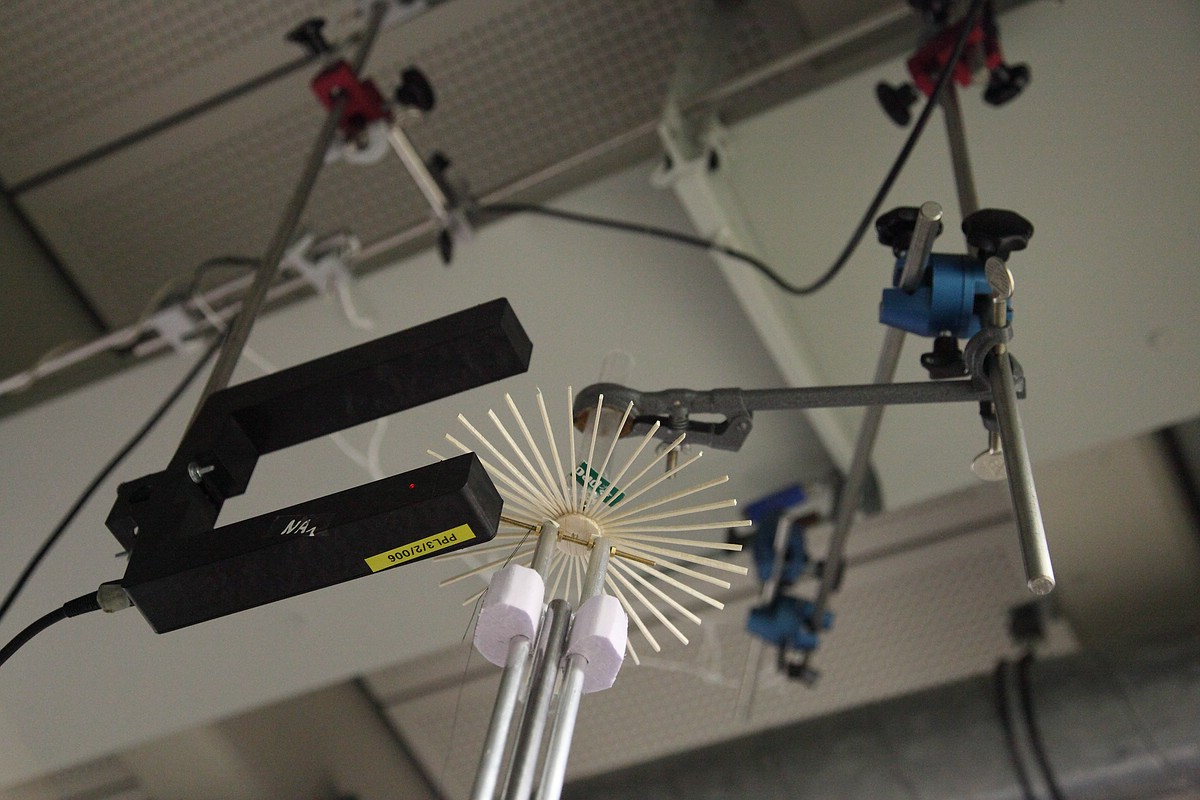
\includegraphics[width=0.8\textwidth]{lichtschranke.jpg}
\end{center}
\vspace{-1.5\baselineskip}
\caption{Das Speichenrad beim Durchgang durch die Lichtschranke}
\label{lichtschranke}
\end{figure}
\begin{figure}[th]
\begin{center}
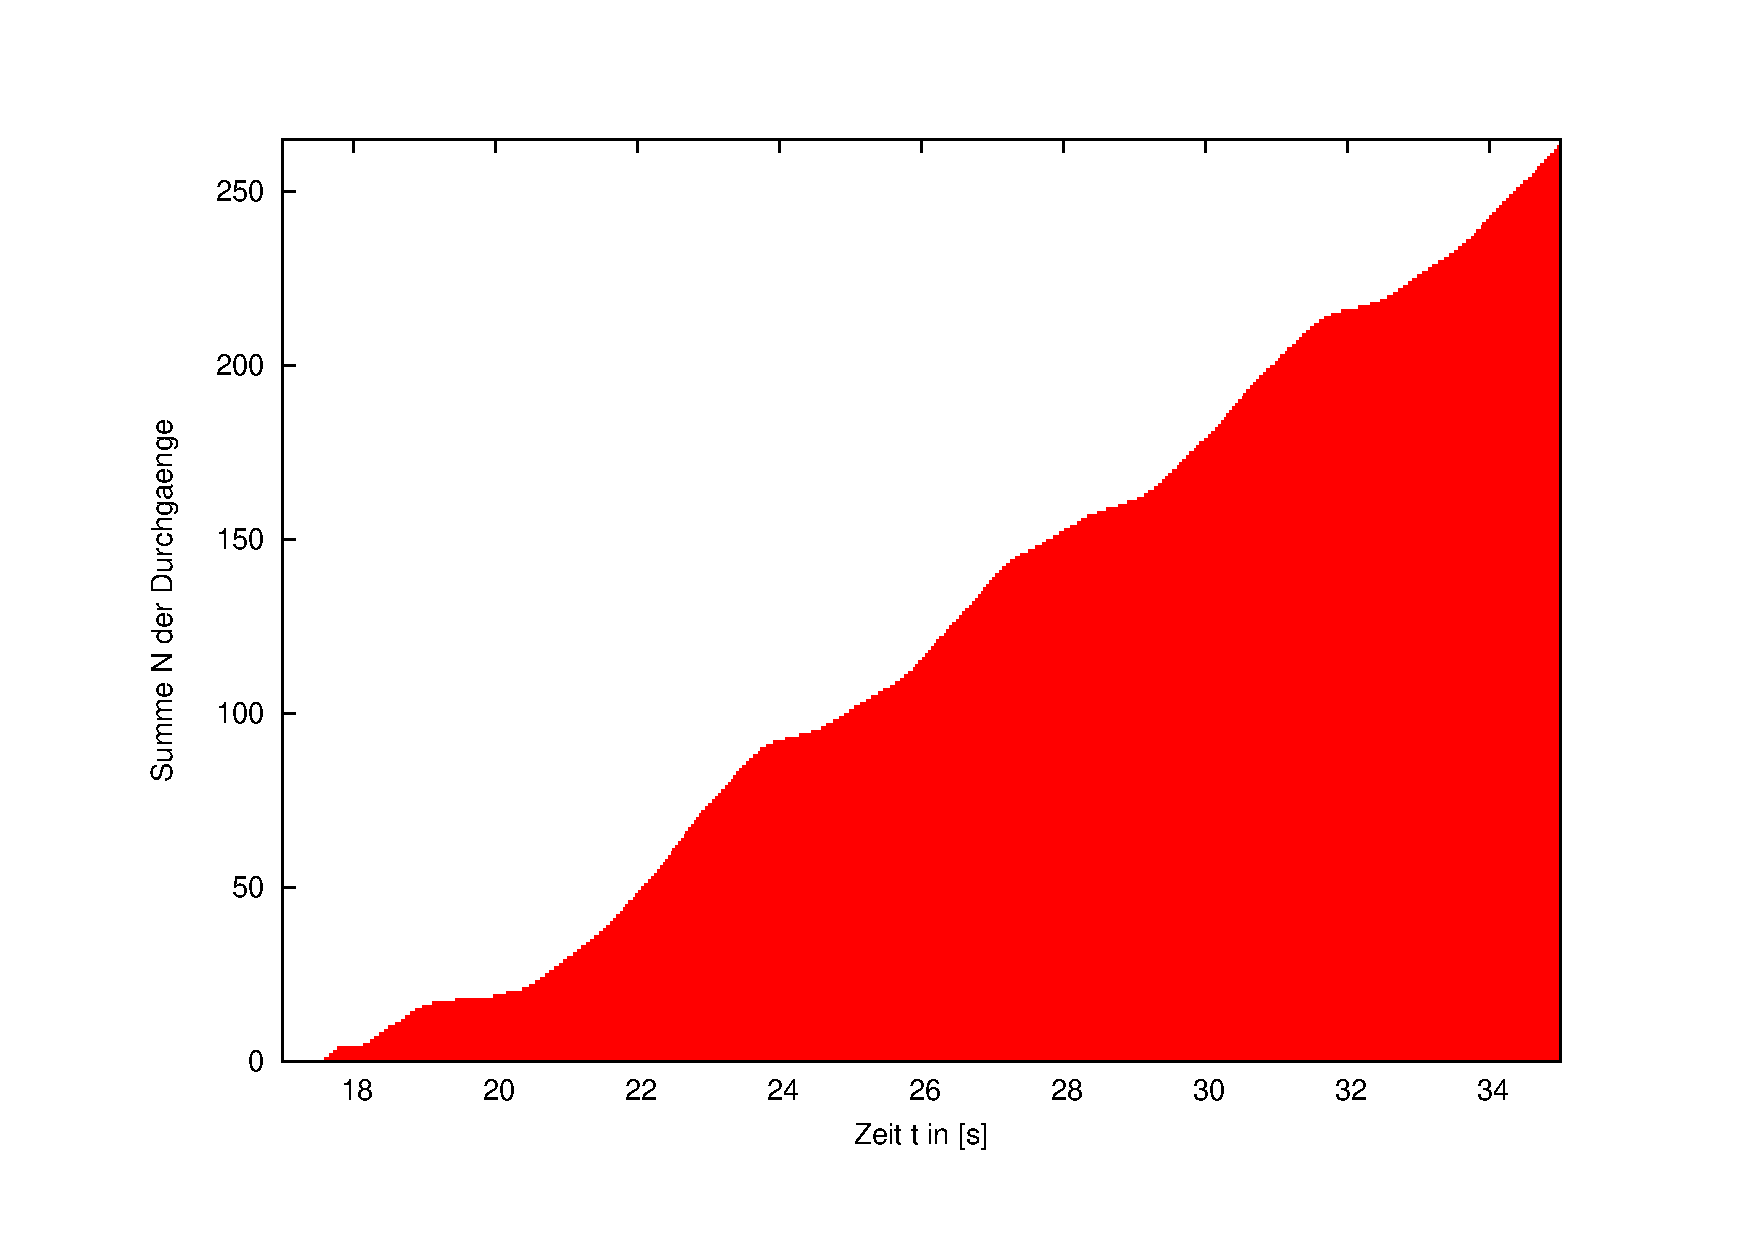
\includegraphics[width=0.8\textwidth]{durchg29-cassy.pdf}
\end{center}
\vspace{-1.5\baselineskip}
\caption{Summe der Durch\"ange durch die Lichtschranke}
\label{durchg29-cassy}
\end{figure}
Zur Aufzeichnung der Drehung des Stabes kam zun\"achst das CASSY Lab System zum Einsatz. Auf H\"ohe der Spitze des Stabes wurde eine Lichtschranke durch Stativstangen an der Deckenkonstruktion verschraubt, welche die Durchg\"ange des Stabes z\"ahlte. Die Ausl\"osung der Lichtschranke sollte durch einen leichten Querstab aus Balsaholz erfolgen. Es stellte sich jedoch heraus, dass dabei nur unzureichende Genauigkeiten bei der Ermittlung der Drehgeschwindikeit erzielt werden konnten, da die Lichtschranke bei dieser Methode nur zweimal pro ganzer Umdrehung ausgel\"ost wird. Deshalb wurde an der Spitze des Stabes ein \glqq Speichenrad\grqq{} installiert. Die einzelnen Speichen hatten dabei einen Abstand von jeweils $10^\circ$. Pro Umdrehung wurde die Schranke also 36 Mal ausgel\"ost. Die L\"ange der einzelnen Speichen wurde so kurz wie m\"oglich gehalten, um das Tr\"agheitsmoment des Stabes nicht unn\"otig zu beeinflussen.
\begin{figure}[ht]
\begin{center}
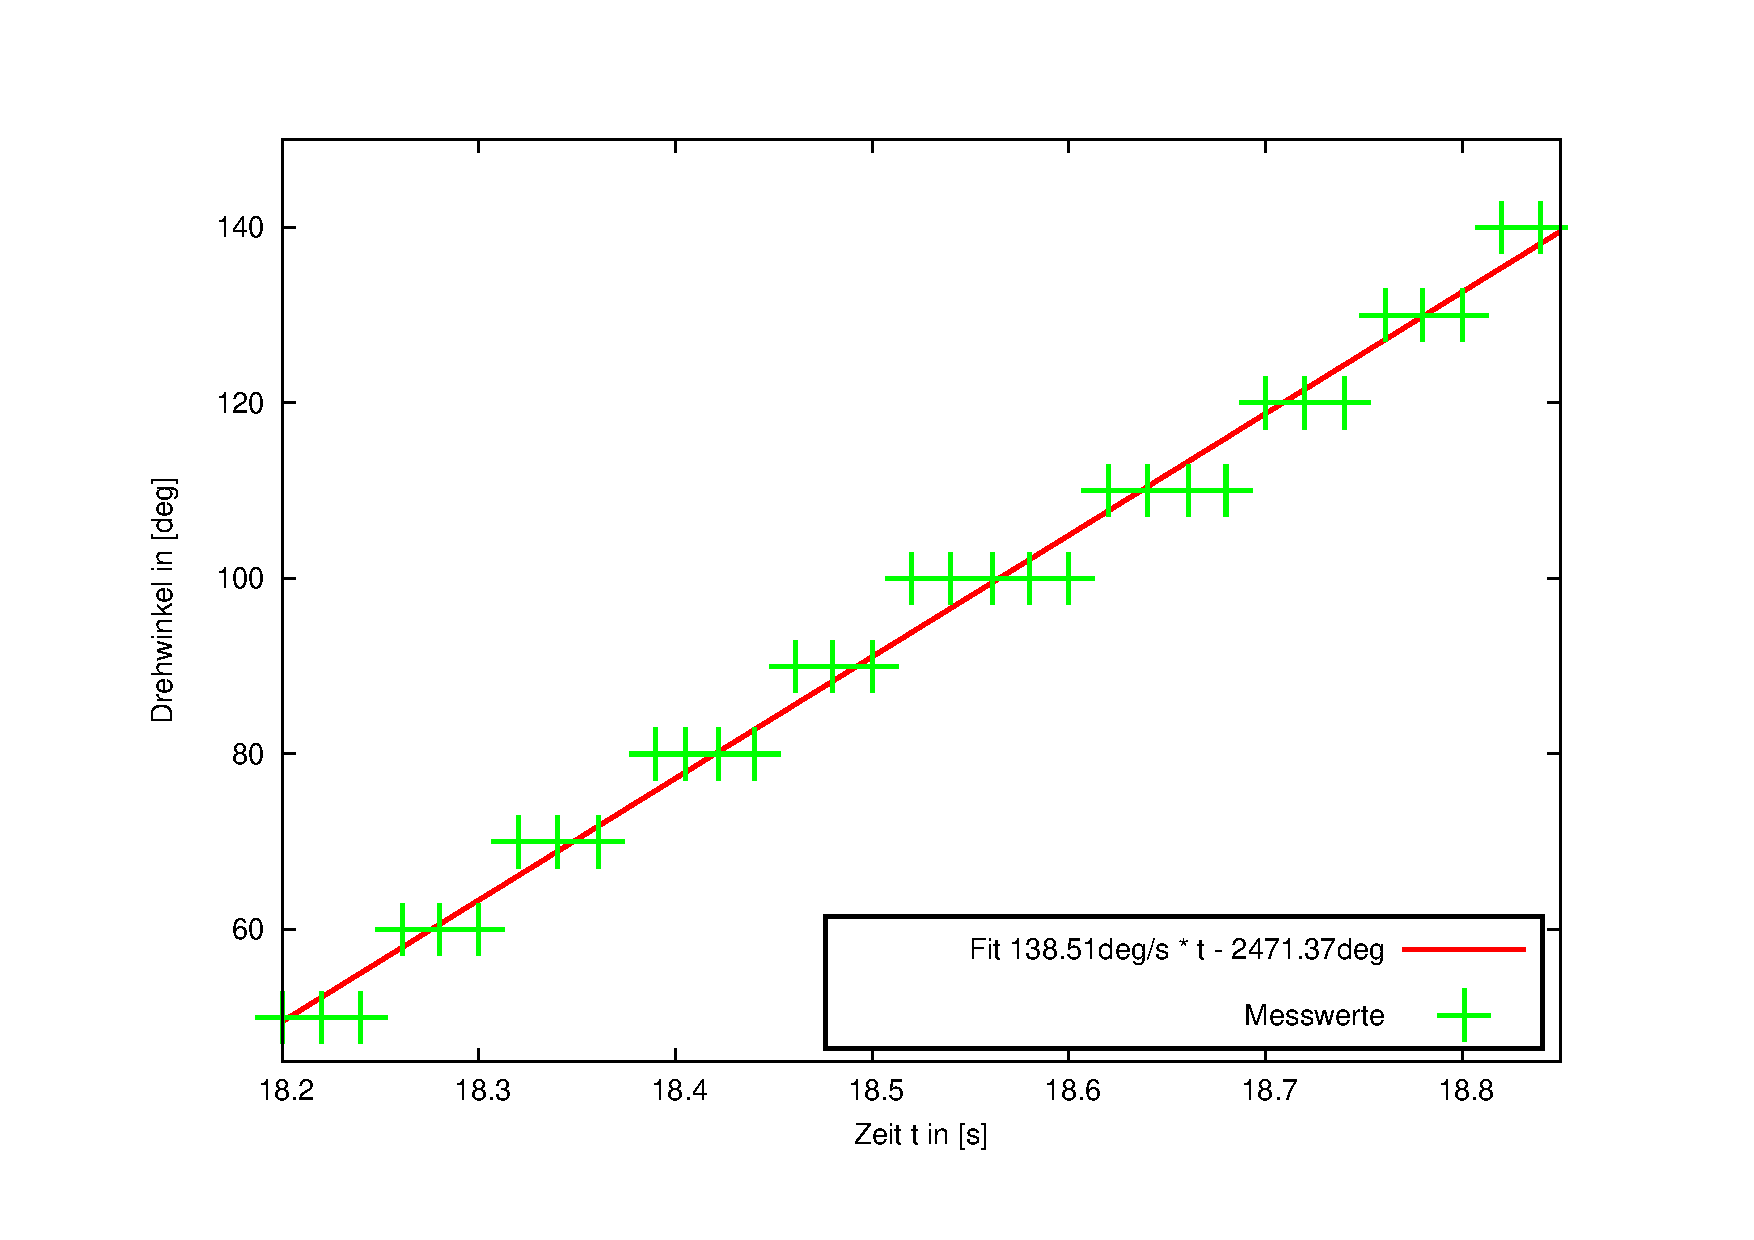
\includegraphics[width=0.99\textwidth]{zeit-winkel29-cassy.pdf}
\end{center}
\vspace{-1.5\baselineskip}
\caption{Geradenfit zur Ermittlung der Winkelgeschwindigkeit}
\label{zeit-winkel29-cassy}
\end{figure}

Die hier ausgewertete Messung wurde am 29.01.2010 durchgef\"uhrt. Der Stab hing bis zum Durchbrennen des Fadens ungef\"ahr 24 Stunden in ausgelenkter Postition. Zu diesem Zeitpunkt wurde bereits der Messingstab verwendet, daher war die Konstruktion auch nicht in Nord-S\"ud-Richtung orientiert, wie dies bei fr\"uheren Versuchen der Fall war. Das CASSY Lab nahm die Durchg\"ange mit einem Messintervall von $20\unit{ms}$ auf. Der folgende Plot (siehe \hypref{Abb.}{durchg29-cassy}) zeigt zun\"achst die aufsummierte Anzahl der Durchg\"ange durch die Lichtschranke seit dem Durchbrennen des Fadens. Bei der Beobachtung der Drehbewegung waren regelm\"a\ss{}ige \"Anderungen der Drehrichtung zu beobachten. Die Lichtschranke konnte zwar nicht zwischen Vor- und R\"uchw\"artsdrehung unterscheiden, jedoch zeigen die Punkte des Graphen mit horizontaler Tangente diese Wechsel, da sich die Drehbewegung hierbei zun\"achst verlangsamte und anschlie\ss{}end nach einem kurzen Stopp wieder in die andere Richtung beschleunigte.

F\"ur die Auswertung konnte somit nur der Bereich vor dem ersten Richtungswechsel verwendet werden, um die Einfl\"usse von au\ss{}en gering zu halten. Nach dem Umrechnen der Zahl der Durchg\"ange in Drehwinkel (1 Durchgang \^{=} $10^\circ$ Drehung) wurde an das \glqq Zeit-Drehwinkel\grqq{} Diagramm (siehe \hypref{Abb.}{zeit-winkel29-cassy}) ein Geradenfit durchgef\"uhrt. Daraus ergibt sich f\"ur die Winkelgeschwindigkeit:
\begin{equation}
\omega\ltext{Cassymessung} = 139\pm 3 \unit{\frac{deg}{s}}
\end{equation}
Eine Umdrehung des hochgeklappten Stabes dauert somit 
\begin{equation}
T_{parallel-Messung}=\frac{360\degr}{139 \unit{\frac{deg}{s}}}=2,59 \unit{s} \ ,
\end{equation}
was knapp zwölf Mal so schnell wie der theoretische Wert von $T_{parallel}= 30,3$ ist (siehe \hypref{Gleichung}{eq:tpara}).\\ \\
Folglich ergibt sich auch f\"ur die resultierende Geschwindigkeit der Erddrehung mit der oben hergeleiteten \hypref{Formel}{eq:grund} ein stark von der Realit\"at abweichender Wert:
\begin{equation}
\omega\ltext{Erde-Messung} = 
\frac{1}{\cos(40,4\degr)}\ 
\frac{139 \unit{\frac{deg}{s}}}{(3,6\ee{-1}) / (9,9\ee{-5}) - 1}
= 5,02\ee{-2} \unit{\frac{deg}{s}}
\end{equation}
Ein Tag dauert somit nach unserer Messung mit dem CASSY Lab nur $7\,170 \unit{s}$ statt $86\,164,1 \unit{s}$.

\FloatBarrier
\subsection{Videomessungen} %Karl
Da die Schwingung der Vorrichtung die Cassymessung fast unbrauchbar machte, wurden weitere Wege gesucht, die bisherigen Versuche dennoch auswertbar zu machen. Als Grundlage sollten hier Videoaufnahmen dienen, die es ermöglichten, die Drehung unmittelbar nach dem Einklappen des Stabes zu beschreiben, bevor die störende Schwingung den Effekt zu stark überlagert. Die zur Verfügung stehenden Mitschnitte wurden ursprünglich nur zu Dokumentationszwecken aufgezeichnet. Dies hatte den Nachteil, dass die Videodateien vor der Auswertung noch stark bearbeitet werden mussten, um Messdaten ablesen zu können. Das Hauptproblem lag in der verzerrten Perspektive des Videos, das von schräg unten aufgenommen wurde (siehe \hypref{Abb.}{Videobearbeitung}). Zur Auswertung wurde mit Hilfe der freien Bildbearbeitungssoftware GIMP wie folgt vorgegangen:\\
Zuerst wurde das Video in seine Einzelbilder zerlegt. Anhand dieser Bilder, im Speziellen der sich drehenden oberen Verbindungsquerstange, wurde durch Fitten einer Ellipse die perspektivische Verzerrung ermittelt. Für das Halbachsenverhältnis dieser Ellipse ergab sich folgender Wert:
\begin{equation}
\frac{a\ltext{groß}}{a\ltext{klein}}=3,21
\end{equation}
Nun wurden die Einzelbilder senkrecht ausgerichtet, also um den Winkel $\alpha$ gedreht (siehe \hypref{Abbildung}{Videobearbeitung} - A) und schließlich um den ermittelten Faktor $3,21$ gestreckt (siehe \hypref{Abbildung}{Videobearbeitung} - B).
\begin{figure}[h]
\begin{center}
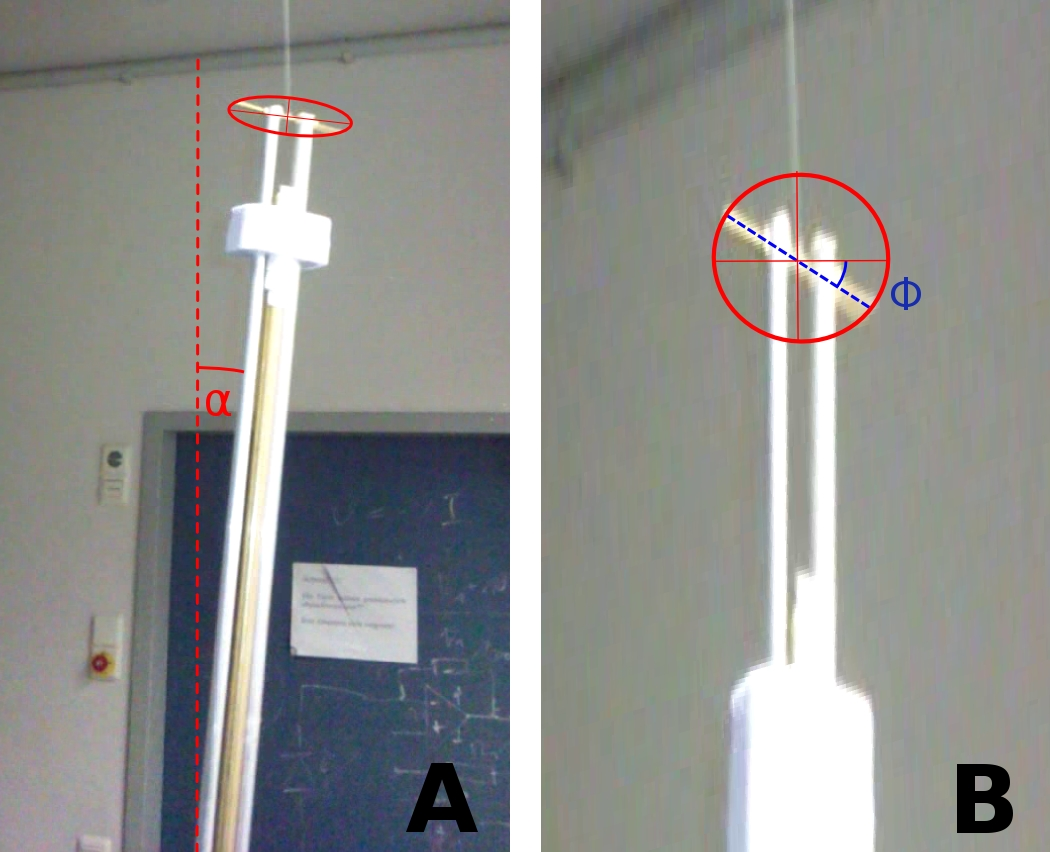
\includegraphics[width=0.8\textwidth]{auswert.jpg}
\end{center}
\vspace{-1.5\baselineskip}
\caption{Bearbeitung der Videoeinzelbilder}
\label{Videobearbeitung}
\end{figure}
Aus diesen Bilddaten konnten nun der Drehwinkel $\phi$ abgelesen werden. Der Fehler dieser Messung lag vor allem in der unterschiedlichen Qualität der Einzelbilder und wurde durch mehrmaliges Messen pro Bild ermittelt.
Da die schon anfänglich erwähnte Schwankung leider sehr schnell nach dem Einklappvorgang ins Gewicht fiel, konnten nur wenige Messpunkte zur Ermittlung der Winkelgeschwindigkeit herangezogen werden.
\begin{figure}[h]
\begin{center}
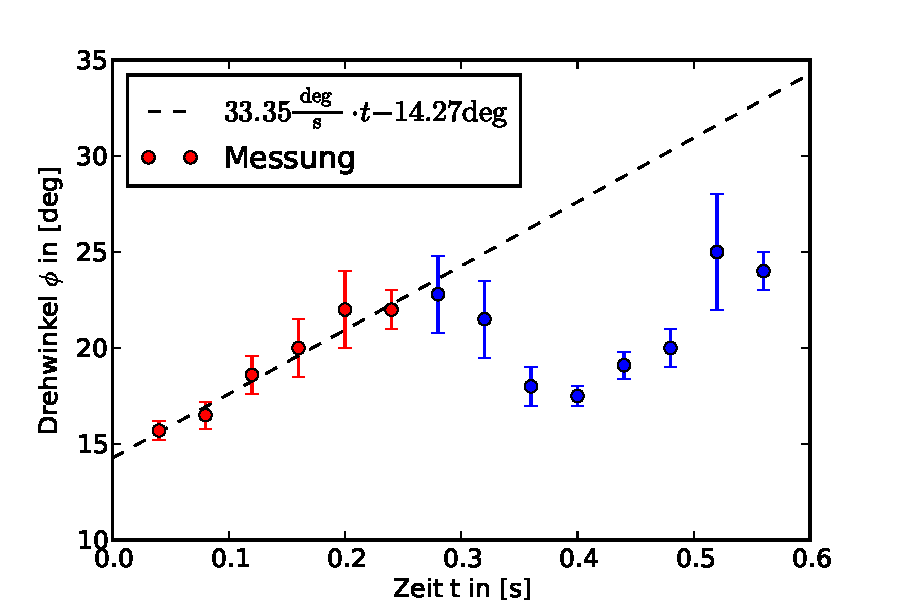
\includegraphics[width=0.8\textwidth]{messung_Video.pdf}
\end{center}
\vspace{-1.5\baselineskip}
\caption{Messergebnisse der Video-Messung}
\label{messung_Video}
\end{figure}
Der zeitliche Abstand der Videoeinzelbilder wurde durch Filmen einer Stoppuhr zu $\Delta t = 0,04\unit{s}$ bestimmt.
Durch einen Geradenfit der ersten sechs Messpunkte wurde die Winkelgeschwindigkeit ermittelt. Es gilt:
\begin{equation}
\omega\ltext{Messung} = 33,35 \unit{\frac{deg}{s}} = 0,582 \unit{s^{-1}}
\end{equation}
Damit ergibt sich mit den bekannten Werten für die Trägheitsmomente folgende Winkelgeschwindigkeit der Erdrotation:
\begin{equation}
\omega\ltext{Erde} = 
\frac{1}{\cos(40,4\degr)}\ 
\frac{\omega\ltext{mess}}{(3,6\ee{-1}) / (9,9\ee{-5}) - 1}
= \frac{1}{4757\unit{s}}
\end{equation}
Die hieraus resultierende Dauer eines Tages weicht weiterhin um einen Faktor von $\frac{1}{18}$ vom wahren Wert ab.


\FloatBarrier
\section{Fehlerquellen und Verbesserungsvorschläge}\label{sec:verbesserung}
 %David: faden, zwei stäbe, kamera von oben, symmetrischerer aufbau
Eine anfängliche, selbstverschuldete Fehlerquelle war die schon erwähnte Wahl eines Eisenstabes und die Verwendung eines Magnets als Haltemechanismus. Das Erdmagnetfeld richtete den Stab wie eine Kompassnadel aus, sodass der erwünschte Effekt nicht messbar war. Durch die Verwendung eines Messingstabs löste sich zwar dieses Problem, allerdings brauchten wir auch einen neuen Einschnappmechanismus. Wir entschlossen uns dazu einen Klettverschluss zu verwenden, was auch einigermaßen gut funktionierte. Jedoch hat dieser immer ein wenig Spiel, weshalb der Stab nicht exakt parallel zur Aufhängeachse arretierte und das reale Trägheitsmoment vom theoretisch berechneten $I_{\textnormal{Aufbau-senkrecht}}$ abwich. Eine Angabe des hierbei verursachten Fehlers ist jedoch nicht wirklich möglich, da die Bestimmung des von den idealen $0^\circ$ abweichenden Winkels zwischen dem Stab und der Drechachse im Moment des Einschnappens und der ersten Drehungen nicht möglich war.

Des Weiteren verursachte auch die Torsion des Fadens Fehler. Einerseits brauchten wir einen Faden, der fest genug ist um den Aufbau zu tragen, andererseits war es natürlich erforderlich, dass er bei der Verdrillung kaum Widerstand leistet und die Drehung nicht sofort bremst. Durch die Wahl des Nylonfadens konnten wir diesen, nicht ohne Weiteres zu quantisierenden Fehler lediglich möglichst minimieren.

Weitere Verbesserungsideen, die uns noch einfielen, aber aufgrund des Zeitmangels nicht mehr durchgeführt werden konnten, sind unter anderem eine neue Halterung des Systems zu konzeptionieren, welche es ermöglicht die Kamera für die Videoanalyse direkt über dem Gestell zu positionieren und somit die Fehler der auftretenden perspektivisch bedingten Winkel zu beseitigen.

Für den generellen Aufbau gibt es noch Spielraum bei dem Einfangmechanismus des Stabes. Neben dem durch den Klettverschluss bedingten Abweich-Winkel des Stabes von der Drehachse, ist es auch sehr wichtig, dass er während des Einklappens nicht in Schwungrichtung zur Seite abdriftet. Anfangs resultierte dies darin, dass der Stab an der Drehachse vorbei schwang, sich wieder fast horizontal ausrichtete und derart weiter oszillierte. Durch die passend gewählte Form der Styroporbremse (siehe \hypref{Abbildung}{lichtschranke}) konnte dies verhindert werden. Dass er genau in der Drehachse auf den Klettverschluss stößt, konnte jedoch nicht erzwungen werden.

Das größte Potential ein besseres Ergebnis zu ermöglichen hat jedoch ein neuer Aufbau, bei dem nicht ein Stab anfangs horizontal ausgerichtet ist und anschließend nach oben schwingt, sondern bei welchem zwei, jeweils an einem Ende freischwingend mit dem Gehäuse verbundene Stäbe derart waagerecht gehalten werden, dass sie in der Ruheposition dann nach unten schwingen können und sich gegenseitig in der Ruhelage bremsen (siehe \hypref{Abbildung}{prinzip2}).

\begin{figure}[h]
\begin{center}
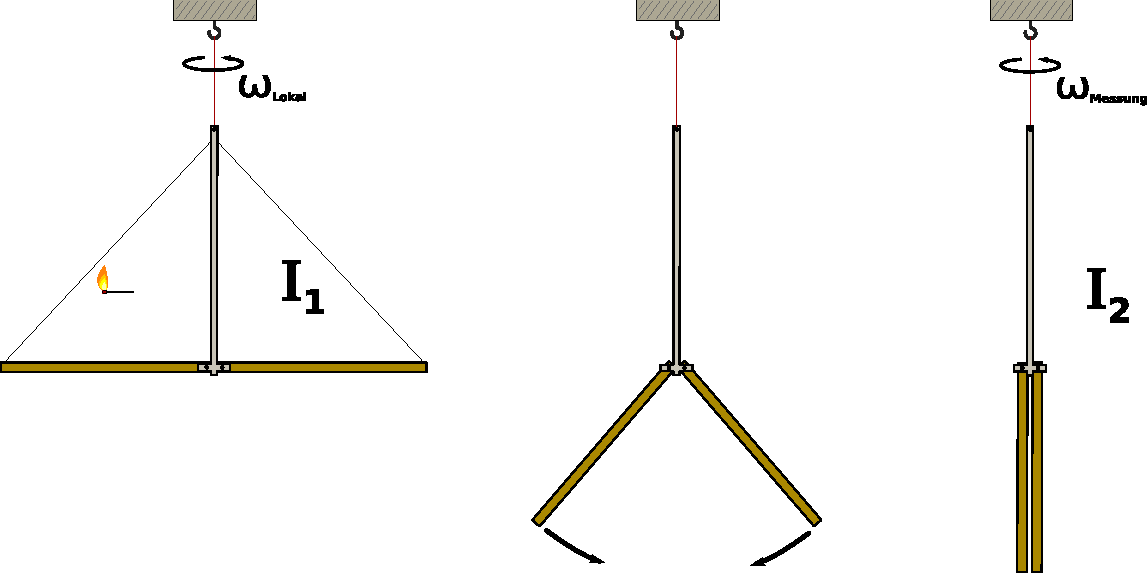
\includegraphics[width=0.8\textwidth]{prinzip-2.pdf}
\end{center}
\vspace{-1.5\baselineskip}
\caption{Alternativer Aufbau}
\label{prinzip2}
\end{figure}


\section{Fazit} %Basti
Dieser Versuch ist ein schönes Beispiel wie es in der Physik Mittel und Wege gibt auch extrem kleine Größen durch ein Experiment zu messen.
Voraussetzung ist aber, neben einem theoretisch richtigen Konzept, die strikte Elimination zahlreicher störender Faktoren.
Der aufgeführte Versuchsaufbau ist zweifelsohne in der Lage die gesuchte Drehbewegung sichtbar zu machen, denn einerseits liegt der theoretische Effekt deutlich im messbaren Bereich, andererseits haben wir die Grenzen der Dimensionierung noch nicht komplett ausgeschöpft.

Unser Problem war allerdings, dass es gleich mehrere signifikante Störgrößen gab und es uns nicht gelungen ist alle innerhalb der zwei Wochen zu identifizieren und zu beheben.
Das Problem mit dem Magneten hätte uns natürlich früher auffallen können.
Einer präzisen, zentralen Aufhängung und der Spielfreiheit unserer Drehgelenke waren allerdings gewisse Grenzen gesetzt.
Bei einigen der in \hypref{Abschnitt}{sec:verbesserung} aufgeführten Versuchsänderungen wären diese Ungenauigkeiten vielleicht weniger kritisch gewesen und wir hätten einen guten Wert erhalten.

Bei einer Abweichung um den Faktor einer Gr"oßenordnung vom theoretischen Wert sind die Fehler nun so groß, dass von einem sicheren Nachweis der Erddrehung natürlich nicht mehr die Rede sein kann.
Wäre es allerdings Galileo Galilei als Begründer der modernen Experimentalphysik gelungen unseren Aufbau ein wenig präziser durchrzuführen, so hätte er den unumstößlichen Beweis in Händen gehabt:
Und sie dreht sich doch!

\end{document}


